\documentclass[11pt,a4paper]{beamer}
\usepackage[utf8]{inputenc}
\usepackage{amsmath}
\usepackage{amsfonts}
\usepackage{amssymb}
\usepackage{graphicx}
\usepackage{verbatim}
\author{Dainius Jocas}
\title{In the Dalvik}

\begin{document}
\frame{\titlepage} 

\begin{frame}[fragile]
\frametitle{Who Calls onCreate()?}

Every activity that we are creating has a method with this notation:
\scriptsize\begin{verbatim}
@Override
protected void onCreate(Bundle savedInstanceState) {
    super.onCreate(savedInstanceState);
    setContentView(R.layout.activity_main);
    // place for your code
}
\end{verbatim} 
\normalsize
Who calls that method?

\end{frame}

\begin{frame}[fragile]
\frametitle{Official documentation on the issue}
\begin{figure}
  \center
  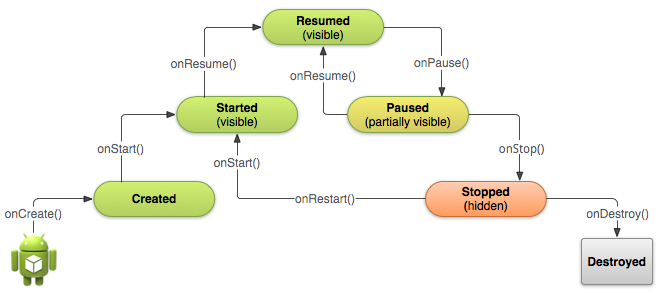
\includegraphics[width=\textwidth]{./images/basiclifecycle.png}
  \caption{Activity lifecycle\footnote{\url{http://developer.android.com/training/basics/activity-lifecycle/starting.html}}}
\end{figure} 
\end{frame}

\begin{frame}[fragile]
\frametitle{class: Activity}

It's not that much surprising that the call is from the extended class:
\scriptsize\begin{verbatim}
final void performCreate(Bundle icicle) {
    onCreate(icicle);
    mVisibleFromClient = !mWindow.getWindowStyle().getBoolean(
            com.android.internal.R.styleable.Window_windowNoDisplay, false);
    mFragments.dispatchActivityCreated();
}
\end{verbatim}
\normalsize

File: ./frameworks/base/core/java/android/app/Activity.java

Line: 5108

Good start!

\end{frame}

\begin{frame}[fragile]
\frametitle{class: Instrumentation}

\scriptsize
\begin{verbatim}
/**
 * Perform calling of an activity's {@link Activity#onCreate}
 * method.  The default implementation simply calls through to that method.
 * 
 * @param activity The activity being created.
 * @param icicle The previously frozen state (or null) to pass through to
 *               onCreate().
 */
public void callActivityOnCreate(Activity activity, Bundle icicle) { 
    ...
    activity.performCreate(icicle);
    ...    
}
\end{verbatim}
\normalsize

File: ./frameworks/base/core/java/android/app/Instrumentation.java

Line: 1080
\end{frame}

\begin{frame}[fragile]
\frametitle{class: ActivityThread}

\scriptsize
\begin{verbatim}
private Activity performLaunchActivity(ActivityClientRecord r, Intent customIntent) {
    ...
    mInstrumentation.callActivityOnCreate(activity, r.state); // line: 2144
    ...
}
private void handleLaunchActivity(ActivityClientRecord r, Intent customIntent) {
    ...
    Activity a = performLaunchActivity(r, customIntent); // line: 2230
    ...
}
\end{verbatim}
\normalsize

File: ./frameworks/base/core/java/android/app/ActivityThread.java 

Line: 2144

\end{frame}

\begin{frame}[fragile]
\frametitle{class: ActivityThread (continued)}

\scriptsize
\begin{verbatim}
public void handleMessage(Message msg) {
switch (msg.what) {
    case LAUNCH_ACTIVITY: {
        Trace.traceBegin(Trace.TRACE_TAG_ACTIVITY_MANAGER, "activityStart");
        ActivityClientRecord r = (ActivityClientRecord)msg.obj;

        r.packageInfo = getPackageInfoNoCheck(
                    r.activityInfo.applicationInfo, r.compatInfo);
        handleLaunchActivity(r, null); // line: 1234
        Trace.traceEnd(Trace.TRACE_TAG_ACTIVITY_MANAGER);
    } break;
    ...
}
\end{verbatim}
\normalsize

Here various types of messages are being responded.

\end{frame}

\begin{frame}[fragile]
\frametitle{class: Handler}

\scriptsize
\begin{verbatim}
    /**
     * Handle system messages here.
     */
    public void dispatchMessage(Message msg) {
        if (msg.callback != null) {
            handleCallback(msg);
        } else {
            if (mCallback != null) {
                if (mCallback.handleMessage(msg)) {
                    return;
                }
            }
            handleMessage(msg);
        }
    }
\end{verbatim}
\normalsize

Callback or not?

File: ./frameworks/base/core/java/android/os/Handler.java

Line: 90
\end{frame}





\begin{frame}[fragile]
\frametitle{class: Looper}



\scriptsize\begin{verbatim}
/**
 * Run the message queue in this thread. Be sure to call
 * {@link #quit()} to end the loop.
 */
public static void loop() {
   ...
   msg.target.dispatchMessage(msg);
   ...
}
\end{verbatim}
\normalsize

File: ./frameworks/base/core/java/android/app/ActivityThread.java

Line: 137
\end{frame}


\begin{frame}[fragile]
\frametitle{class: ActivityThread}
Once again we are in this class, but it is because of the experiment.
\scriptsize
\begin{verbatim}
public static void main(String[] args) {
    ...
    Looper.loop(); // line: 5048
    ...
}
\end{verbatim}
\normalsize

\end{frame}


\begin{frame}[fragile]
\frametitle{class Method}
File: ./libcore/luni/src/main/java/java/lang/reflect/Method.java

\tiny
\begin{verbatim}
/**
 * This class represents a method. Information about the method can be accessed,
 * and the method can be invoked dynamically.
 */
...
public Object invoke(Object receiver, Object... args)
        throws IllegalAccessException, IllegalArgumentException, InvocationTargetException {
    if (args == null) {
        args = EmptyArray.OBJECT;
    }
    return invokeNative(receiver, args, declaringClass, parameterTypes, returnType, slot, flag);
}

private native Object invokeNative(Object obj, Object[] args, Class<?> declaringClass,
        Class<?>[] parameterTypes, Class<?> returnType, int slot, boolean noAccessCheck)
                throws IllegalAccessException, IllegalArgumentException,
                        InvocationTargetException; // line: 528
\end{verbatim}
\normalsize

So far, so good, but now the real mess begins.
\end{frame}


\begin{frame}[fragile]
\frametitle{Native Method}

\scriptsize
\begin{verbatim}
File: ./dalvik/vm/native/java_lang_reflect_Method.cpp

/*
 * private Object invokeNative(Object obj, Object[] args, Class declaringClass,
 *   Class[] parameterTypes, Class returnType, int slot, boolean noAccessCheck)
 *
 * Invoke a static or virtual method via reflection.
 */
static void Dalvik_java_lang_reflect_Method_invokeNative(const u4* args,
    JValue* pResult)
{
\end{verbatim}
\normalsize

What happens here is that runtime didn't find a class to which the needed method belongs. 

\end{frame}

\begin{frame}[fragile]
\frametitle{class: ZygoteInit}
\scriptsize
\begin{verbatim}
file: ./frameworks/base/core/java/com/android/internal/os/ZygoteInit.java
/**
 * Startup class for the zygote process.
 *
 * Pre-initializes some classes, and then waits for commands on a UNIX domain
 * socket. Based on these commands, forks off child processes that inherit
 * the initial state of the VM.
 ...
public static void main(String argv[]) {
    ...
    } catch (MethodAndArgsCaller caller) { //line 559
	...
	
\end{verbatim}
\normalsize
\end{frame}

\begin{frame}[fragile]
\frametitle{Grey zone}

file: ./libcore/dalvik/src/main/java/dalvik/system/NativeStart.java
\scriptsize
\begin{verbatim}
/**
 * Dummy class used during JNI initialization.  The JNI functions want
 * to be able to create objects, and the VM needs to discard the references
 * when the function returns.  That gets a little weird when we're
 * calling JNI functions from the C main(), and there's no Java stack frame
 * to hitch the references onto.
 *
 * Rather than having some special-case code, we create this simple little
 * class and pretend that it called the C main().
 *
 * This also comes in handy when a native thread attaches itself with the
 * JNI AttachCurrentThread call.  If they attach the thread and start
 * creating objects, we need a fake frame to store stuff in.
 */
\end{verbatim}
dalvik.system.NativeStart.main(Native Method)

In other words: smoke and mirrors.

\end{frame}

\begin{frame}[fragile]

What about suggestions for future work?

\end{frame}

\end{document}